% !TEX program = pdflatex
\documentclass[11pt,a4paper]{article}

\usepackage[T1]{fontenc}
\usepackage[utf8]{inputenc}
\usepackage{lmodern}
\usepackage[english]{babel}
\usepackage[margin=2.4cm]{geometry}
\usepackage{amsmath,amssymb}
\usepackage{graphicx}
\usepackage{booktabs}
\usepackage{tabularx}
\usepackage{multirow}
\usepackage{xcolor}
\usepackage{caption}
\usepackage{subcaption}
\usepackage{listings}
\usepackage{enumitem}
\usepackage{microtype}
\usepackage{pgfplots}
\pgfplotsset{compat=1.18}
\usepackage[numbers,sort&compress]{natbib}
\usepackage[colorlinks=true,linkcolor=blue!55!black,citecolor=blue!55!black,urlcolor=blue!55!black]{hyperref}

\graphicspath{{figs/}}

% Spanish names while the (English) hyphenation patterns are loaded.
\addto\captionsenglish{%
  \renewcommand{\abstractname}{Resumen}%
  \renewcommand{\refname}{Referencias}%
  \renewcommand{\figurename}{Figura}%
  \renewcommand{\tablename}{Tabla}%
  \renewcommand{\appendixname}{Ap\'endice}%
  \renewcommand{\contentsname}{\'Indice}%
}

\captionsetup{font=small,labelfont=bf}
\setlist{itemsep=1pt,topsep=2pt}

\definecolor{rustorange}{HTML}{B7410E}
\lstdefinestyle{rust}{
  basicstyle=\ttfamily\footnotesize,
  keywordstyle=\color{rustorange}\bfseries,
  commentstyle=\color{gray!80!black}\itshape,
  stringstyle=\color{teal!80!black},
  numbers=left, numberstyle=\tiny\color{gray}, numbersep=6pt,
  frame=single, framerule=0.3pt, rulecolor=\color{gray!50},
  backgroundcolor=\color{gray!4},
  breaklines=true, columns=fullflexible, keepspaces=true,
  showstringspaces=false, tabsize=2, upquote=true,
  literate={->}{{$\rightarrow$}}2 {<-}{{$\leftarrow$}}2,
}
\lstset{style=rust}

% Generated by scripts/make_report.py -- do not edit.
\newcommand{\AucIsl}{0.711}
\newcommand{\AucPan}{0.683}
\newcommand{\AucSeq}{0.683}
\newcommand{\BdivIsl}{0.899}
\newcommand{\BdivPan}{0.697}
\newcommand{\BdivSeq}{0.697}
\newcommand{\BenchEvalsPerSecond}{606.6}
\newcommand{\BenchMillionsCells}{2.12}
\newcommand{\BenchMillionsSteps}{12.13}
\newcommand{\BenchStepsPerSecond}{12131175}
\newcommand{\BytesIsl}{19.0}
\newcommand{\BytesPan}{0.0}
\newcommand{\BytesSeq}{0.0}
\newcommand{\ClassicCompactness}{0.0053}
\newcommand{\ClassicComplexity}{0.4824}
\newcommand{\ClassicDx}{-2}
\newcommand{\ClassicDy}{2}
\newcommand{\ClassicFitness}{0.186}
\newcommand{\ClassicMatch}{1.0000}
\newcommand{\ClassicMobility}{0.0250}
\newcommand{\ClassicNewCells}{24652}
\newcommand{\ClassicPeriod}{104}
\newcommand{\ClassicSpeed}{0.0272}
\newcommand{\EfficiencyIsl}{78.4}
\newcommand{\EvalsIsl}{19919}
\newcommand{\EvalsPan}{20322}
\newcommand{\EvalsSeq}{20322}
\newcommand{\FinalIsl}{$0.737 \pm 0.012$}
\newcommand{\FinalIslMean}{0.737}
\newcommand{\FinalPan}{$0.714 \pm 0.014$}
\newcommand{\FinalPanMean}{0.714}
\newcommand{\FinalSeq}{$0.714 \pm 0.014$}
\newcommand{\FinalSeqMean}{0.714}
\newcommand{\MigFiveAuc}{0.711}
\newcommand{\MigFiveBdiv}{0.899}
\newcommand{\MigFiveBest}{$0.737 \pm 0.012$}
\newcommand{\MigFiveKb}{19.0}
\newcommand{\MigFiveMsgs}{379}
\newcommand{\MigFiveTime}{6.05}
\newcommand{\MigNoneAuc}{0.703}
\newcommand{\MigNoneBdiv}{0.869}
\newcommand{\MigNoneBest}{$0.736 \pm 0.008$}
\newcommand{\MigNoneKb}{14.2}
\newcommand{\MigNoneMsgs}{320}
\newcommand{\MigNoneTime}{5.51}
\newcommand{\MigTwentyAuc}{0.702}
\newcommand{\MigTwentyBdiv}{0.877}
\newcommand{\MigTwentyBest}{$0.737 \pm 0.012$}
\newcommand{\MigTwentyKb}{15.2}
\newcommand{\MigTwentyMsgs}{332}
\newcommand{\MigTwentyTime}{5.95}
\newcommand{\MsgsIsl}{379}
\newcommand{\MsgsPan}{0}
\newcommand{\MsgsSeq}{0}
\newcommand{\OverheadBytesPerEval}{0.9784}
\newcommand{\PortfolioBalancedFit}{0.484}
\newcommand{\PortfolioBalancedSpeed}{0.333}
\newcommand{\PortfolioBuilderFit}{0.861}
\newcommand{\PortfolioBuilderSpeed}{0.200}
\newcommand{\PortfolioMoverFit}{0.633}
\newcommand{\PortfolioMoverSpeed}{0.707}
\newcommand{\PortfolioWeaverFit}{0.707}
\newcommand{\PortfolioWeaverSpeed}{0.005}
\newcommand{\PvalueDivMigNoneFive}{0.1875}
\newcommand{\PvalueIslPan}{0.0625}
\newcommand{\PvalueIslSeq}{0.0625}
\newcommand{\PvalueMigFiveTwenty}{0.5000}
\newcommand{\PvalueMigNoneFive}{1.0000}
\newcommand{\SingleBalancedBest}{$0.5179 \pm 0.0004$}
\newcommand{\SingleBalancedBestMean}{0.518}
\newcommand{\SingleBalancedBestSd}{0.0004}
\newcommand{\SingleWeaverBest}{$0.7041 \pm 0.0444$}
\newcommand{\SingleWeaverBestMean}{0.704}
\newcommand{\SingleWeaverBestSd}{0.0444}
\newcommand{\SpeedupIsl}{3.14}
\newcommand{\SpeedupPan}{2.41}
\newcommand{\TSeventyIsl}{1.26}
\newcommand{\TSeventyPan}{2.15}
\newcommand{\TSeventySeq}{6.19}
\newcommand{\WallIsl}{6.05}
\newcommand{\WallIslSd}{1.11}
\newcommand{\WallPan}{7.88}
\newcommand{\WallPanSd}{1.47}
\newcommand{\WallSeq}{18.98}
\newcommand{\WallSeqSd}{1.09}


\title{\bfseries Evoluci\'on gen\'etica distribuida de aut\'omatas\\
de Langton generalizados: dise\~no e implementaci\'on\\
en Rust, con evaluaci\'on emp\'irica}
\author{Proyecto \emph{Distributed Langton Ant}\\[2pt]
\small c\'odigo, datos y figuras reproducibles en el repositorio del proyecto}
\date{Octubre de 2026}

\begin{document}
\maketitle

\begin{abstract}
\noindent
La hormiga de Langton es un aut\'omata celular m\'inimo capaz de generar
conducta emergente: tras unos diez mil pasos construye una ``autopista''
peri\'odica.  En este trabajo estudiamos una generalizaci\'on del modelo
(aut\'omatas de Turing bidimensionales o \emph{turmites}) y la evoluimos con un
algoritmo gen\'etico distribuido de modelo de islas, implementado \'integramente
en Rust y sin dependencias externas.  Cada isla es un proceso independiente que
se comunica con sus vecinas por TCP en un anillo, migrando asincr\'onicamente
los dos mejores genomas cada cierto n\'umero de generaciones, mientras un
monitor recolecta telemetr\'ia.  La aptitud combina cuatro se\~nales
normalizadas ---movilidad, densidad, complejidad morfol\'ogica y uso de
color--- y el espacio de b\'usqueda contiene $18^{6}\approx3.4\times10^{7}$
reglas para $S=2$ estados y $C=3$ colores.  Sobre cinco semillas, el cl\'uster de
cuatro islas obtiene una aptitud final de \FinalIsl{} frente a
\FinalPan{} del modelo panm\'ictico y \FinalSeq{} del secuencial, con una
aceleraci\'on de $\SpeedupIsl\times$ respecto de este \'ultimo y una eficiencia
paralela del $\EfficiencyIsl\%$.  El portafolio heterog\'eneo redescubre
cualitativamente cuatro familias de conducta (transportador, constructor,
tejedor y equilibrado), incluida una cinta transportadora de per\'iodo $9$;
sobre la regla cl\'asica, el detector recupera la autopista de per\'iodo $104$.  El art\'iculo documenta el modelo, el algoritmo,
el protocolo de red, la metodolog\'ia experimental y todos los resultados
num\'ericos; el c\'odigo y los datos permiten regenerar cada tabla y figura.

\vspace{0.6em}
\noindent\textbf{Palabras clave:} hormiga de Langton, turmite, aut\'omatas
celulares, algoritmos gen\'eticos, computaci\'on distribuida, modelo de islas,
Rust, vida artificial.

\vspace{1.0em}
\noindent\textbf{Abstract}
\small
Langton's ant is a minimal cellular automaton that produces emergent behaviour:
after roughly ten thousand steps it builds a periodic ``highway''.  We study a
generalization of the model (two-dimensional Turing machines, or \emph{turmites})
and evolve it with a distributed island-model genetic algorithm written entirely
in Rust with no external dependencies.  Each island is an independent process
that talks to its neighbours over TCP in a ring, asynchronously migrating its two
best genomes every few generations while a monitor collects telemetry.  Fitness
combines four normalized signals---mobility, density, morphological complexity
and colour usage---over a search space of $18^{6}\approx3.4\times10^{7}$ rules for
$S=2$ states and $C=3$ colours.  Across five seeds the four-island cluster
reaches a final fitness of \FinalIsl, versus \FinalPan{} for the panmictic
model and \FinalSeq{} for the sequential one, with a $\SpeedupIsl\times$ speedup
over the latter and $\EfficiencyIsl\%$ parallel efficiency.  A heterogeneous
portfolio rediscovers four qualitatively different behaviours (conveyor,
builder, weaver and balanced), including a period-$9$ conveyor belt, while the
detector recovers the classic period-$104$ highway of the baseline rule.  We document the model, the algorithm, the wire protocol,
the experimental methodology and every numerical result; code and data suffice
to regenerate each table and figure.
\normalsize
\end{abstract}

\tableofcontents

% ===========================================================================
\section{Introducci\'on}
% ===========================================================================

Los aut\'omatas celulares son modelos de c\'omputo en los que una regla local,
aplicada de forma sincr\'onica sobre una rejilla, produce patrones globales que
a menudo no pueden deducirse de la regla misma \citep{wolfram2002}.  La
\emph{hormiga de Langton}, propuesta por Christopher Langton como ejemplo
m\'inimo de vida artificial \citep{langton1986}, es uno de los casos m\'as
citados: una ``hormiga'' ocupa una celda de una rejilla binaria, lee el color,
lo invierte, gira a la derecha si la celda era blanca y a la izquierda si era
negra, y avanza.  Con esa regla de dos l\'ineas el sistema exhibe tres fases:
simetr\'ia inicial, caos aparente y, alrededor del paso $10^{4}$, una
\emph{autopista} peri\'odica de $104$ pasos que se desplaza indefinidamente en
diagonal \citep{gale1995}.

La generalizaci\'on natural, introducida por el propio Langton, permite $S$
estados internos y $C$ colores de celda, y se conoce como \emph{turmite}
\citep{langton1986,gale1995}.  El espacio de reglas crece muy r\'apido y la
mayor\'ia de sus puntos produce conductas triviales, peri\'odicas o
degeneradas; encontrar reglas ``interesantes'' a mano es inviable.  Esto
convierte al modelo en un banco de pruebas ideal para b\'usqueda evolutiva:
la funci\'on de aptitud puede premiar propiedades observables de la
trayectoria y del patr\'on, y el resultado es una regla de f\'acil lectura y
verificaci\'on.

Este trabajo aborda dos preguntas.  La primera es de \emph{dise\~no}: ¿qu\'e
familias de conducta emergente pueden descubrirse con una aptitud multiobjetivo
sencilla y un algoritmo gen\'etico est\'andar?  La segunda es de
\emph{ingenier\'ia}: ¿qu\'e se gana al distribuir la poblaci\'on en islas
que intercambian individuos por red, en t\'erminos de tiempo, calidad y
diversidad?  Para responderlas construimos un sistema completo y lo evaluamos
con un protocolo reproducible de cinco semillas.

\paragraph{Contribuciones.}
\begin{enumerate}
  \item Un simulador determinista de turmites con rejilla dispersa y sin l\'imites
        artificiales, y un detector de autopistas que \emph{verifica} la
        periodicidad re-simulando y comparando el patr\'on trasladado, en lugar
        de confiar s\'olo en la recurrencia del estado local.
  \item Una aptitud multiobjetivo de cuatro componentes normalizadas
        (movilidad, densidad, complejidad de vecindades $3\times3$ y uso de
        color), con perfiles de pesos que inducen conductas cualitativamente
        distintas.
  \item Un algoritmo gen\'etico de islas as\'incrono sobre TCP: cuatro procesos,
        topolog\'ia en anillo, migraci\'on de los dos mejores genomas,
        inyecci\'on selectiva y monitor de telemetr\'ia, sin dependencias
        externas.
  \item Una implementaci\'on en Rust (unos 3\,100 l\'ineas) que incluye
        planificador de hilos con \texttt{std::thread::scope}, codificador PNG
        propio y una interfaz de l\'inea de comandos con nueve subcomandos.
  \item Una evaluaci\'on emp\'irica con presupuestos iguales, cinco semillas,
        pruebas de permutaci\'on exactas y todos los datos crudos versionados
        junto al c\'odigo.
\end{enumerate}

El resto del art\'iculo se organiza as\'i: la Secci\'on~\ref{sec:related} revisa
el trabajo relacionado; la Secci\'on~\ref{sec:model} define el modelo y el
detector de autopistas; la Secci\'on~\ref{sec:fitness} describe la aptitud; la
Secci\'on~\ref{sec:ga} presenta el algoritmo y la arquitectura distribuida; la
Secci\'on~\ref{sec:method} detalla la metodolog\'ia; la
Secci\'on~\ref{sec:results} reporta los resultados; la
Secci\'on~\ref{sec:discussion} los discute y la
Secci\'on~\ref{sec:conclusions} concluye.

% ===========================================================================
\section{Trabajo relacionado}\label{sec:related}
% ===========================================================================

\paragraph{La hormiga y sus generalizaciones.}
Langton introdujo la hormiga como ejemplo de c\'omputo emergente en el borde
del caos \citep{langton1986,langton1990}.  \citet{gale1995} estudiaron las
autopistas, conjeturaron que toda configuraci\'on finita acaba construyendo una
y analizaron turmites con m\'as estados y colores.  La conjetura de la autopista
sigue abierta para la regla cl\'asica, aunque se sabe que la trayectoria es no
acotada; para versiones generalizadas se han construido reglas universalmente
computacionales y se ha demostrado que predecir la trayectoria es
computacionalmente dif\'icil \citep{gajardo2002}.  Trabajos recientes siguen
descubriendo familias de autopistas en espacios de reglas generalizados, lo que
confirma que el modelo dista de estar agotado.

\paragraph{Evoluci\'on de aut\'omatas celulares.}
La evoluci\'on de reglas celulares con algoritmos gen\'eticos tiene una larga
tradici\'on; el trabajo de \citet{mitchell1993} sobre aut\'omatas que realizan
c\'omputo es el ejemplo can\'onico de c\'omo la selecci\'on puede descubrir
reglas no triviales en un espacio discreto.  Nuestro enfoque difiere en el
objetivo---no buscamos una funci\'on computacional sino morfolog\'ias y
trayectorias---y en la escala: reglas diminutas ($S\!\cdot\!C=6$ entradas) y
simulaciones cortas ($10^{4}$ pasos), lo que permite muchas evaluaciones.

\paragraph{Calidad y diversidad.}
La presi\'on por diversidad conductual se inspira en la b\'usqueda de novedad
\citep{lehman2011}: en lugar de premiar s\'olo el mejor valor escalar,
registramos cu\'antas conductas distintas coexisten.  Nuestra m\'etrica es m\'as
modesta (cuatro componentes cuantizadas) pero cumple la misma funci\'on de
diagn\'ostico y se reporta en todas las tablas.

\paragraph{Algoritmos gen\'eticos paralelos y distribuidos.}
El modelo de islas es una de las formas cl\'asicas de paralelizar un algoritmo
gen\'etico \citep{tanese1989,cantupaz1998,alba2002}.  La migraci\'on peri\'odica
de individuos entre subpoblaciones equilibra exploraci\'on y explotaci\'on, y su
efecto depende de la topolog\'ia, del intervalo y del n\'umero de migrantes
\citep{whitley1998island}.  Frente a la alternativa panm\'ictica ---una sola
poblaci\'on evaluada en paralelo--- el modelo de islas preserva diversidad
gen\'etica y permite escalar a m\'aquinas f\'isicamente separadas.  Aqu\'i
implementamos la variante as\'incrona: no hay barrera entre generaciones y los
mensajes se reciben cuando llegan, lo que evita sincronizar procesos lentos a
costa de perder reproducibilidad bit a bit.

\paragraph{Rust.}
La implementaci\'on usa s\'olo la biblioteca est\'andar \citep{klabnik2023}:
hilos con \texttt{scope}, canales \texttt{mpsc}, TCP y escritura de CSV.  La
ausencia de dependencias hace que el binario sea trivial de compilar y de
auditar, propiedad valiosa para un experimento que aspira a ser reproducible
\citep{peng2011}.

% ===========================================================================
\section{Modelo}\label{sec:model}
% ===========================================================================

\subsection{Aut\'omata de Turing bidimensional}

Un turmite se define por la tupla $(S,C,\delta)$, donde $S=\{0,\dots,S-1\}$ es
el conjunto de estados internos de la hormiga, $C=\{0,\dots,C-1\}$ el de colores
de celda y
\begin{equation}
  \delta : S\times C \;\longrightarrow\; C\times\{\mathrm{L},\mathrm{R},\mathrm{U}\}\times S
\end{equation}
es la tabla de reglas.  En cada paso, con la hormiga en la posici\'on $(x,y)$,
direcci\'on $d\in\{\mathrm{N},\mathrm{E},\mathrm{S},\mathrm{W}\}$ y estado $s$,
se lee el color $c$ de la celda, se escribe $\delta(s,c).c'$, se gira
$\delta(s,c).t$ ($90^\circ$ a la izquierda, a la derecha o $180^\circ$), se
avanza una celda en la nueva direcci\'on y se adopta el estado
$\delta(s,c).s'$.  La regla cl\'asica de Langton es el caso $S=2$, $C=2$ con
\begin{center}
\begin{tabular}{ccc}
\toprule
$(s,c)$ & escritura, giro, estado & hex \\
\midrule
$(0,0)$ & $1$, derecha, $0$ & \texttt{010100} \\
$(0,1)$ & $0$, izquierda, $0$ & \texttt{000000} \\
$(1,\cdot)$ & no alcanzable & \texttt{000000} \\
\bottomrule
\end{tabular}
\end{center}
es decir, el genoma \texttt{010100000000000000000000}.  Para $S=2$ y $C=3$ el
n\'umero de reglas es
\begin{equation}
  |\mathcal{G}| = \bigl(C\cdot 3\cdot S\bigr)^{S\cdot C} = 18^{6} = 34\,012\,224,
\end{equation}
un espacio lo bastante grande para que la b\'usqueda exhaustiva sea costosa y lo
bastante peque\~no para que un genoma quepa en 36 caracteres hexadecimales.

\subsection{Codificaci\'on del genoma}

Cada entrada de la tabla se serializa en tres bytes: color escrito, giro
($0=\mathrm{L},1=\mathrm{R},2=\mathrm{U}$) y estado siguiente.  Un genoma de
$S\cdot C$ entradas ocupa $6SC$ caracteres hexadecimales; esta representaci\'on
es la que viaja por la red y la que se escribe en los archivos de resultados, de
modo que cualquier individuo puede re-evaluarse con un solo comando; el formato de los mensajes de migraci\'on se
describe en la Secci\'on~\ref{sec:ga}.

\subsection{Simulaci\'on con rejilla dispersa}

La rejilla se implementa como un \texttt{HashMap} de bloques de $32\times32$
celdas; s\'olo se materializan los bloques visitados.  Leer una celda no
visitada devuelve el color $0$ sin asignar memoria, y la huella es proporcional
al \'area efectivamente explorada, no al desplazamiento.  Esto permite simular
autopistas que se alejan indefinidamente sin fijar un toro ni un l\'imite
arbitrario, algo esencial porque varias conductas \'optimas son precisamente
aquellas que escapan.  La simulaci\'on es determinista: misma regla, mismas
condiciones iniciales, misma traza.

\subsection{Detecci\'on y verificaci\'on de autopistas}

Decir que una regla ``forma una autopista'' requiere algo m\'as que observar que
la hormiga se repite.  Definimos una autopista como una \emph{periodicidad
espacio-temporal}: existen un per\'iodo $p$ y una deriva constante
$(\Delta x,\Delta y)$ tales que
\begin{enumerate}
  \item la secuencia de estados locales $(d_t,s_t)$ es peri\'odica de per\'iodo
        $p$;
  \item el desplazamiento entre $t$ y $t+p$ es el mismo $(\Delta x,\Delta y)$
        para todo $t$ en la ventana final;
  \item el patr\'on construido en $t-p$, trasladado por $(\Delta x,\Delta y)$,
        coincide con el patr\'on en $t$ en una ventana de radio $128$ alrededor
        de la posici\'on anterior de la hormiga.
\end{enumerate}
La condici\'on~(3) es la que separa una autopista real de una coincidencia del
estado local.  Para verificarla se re-simula hasta $t-p$ y se compara celda a
celda con el estado final trasladado.  Los periodos candidatos se buscan
probando la periodicidad de los \'ultimos $4p$ s\'imbolos para todo
$p\le\min(T/3,4096)$; se aceptan como mucho ocho candidatos y se exige
coincidencia exacta y al menos $50$ celdas comparadas.  Con la regla cl\'asica y
$T=120\,000$ el detector recupera $p=104$, deriva $(-2,2)$ y coincidencia
$1.0$ (Tabla~\ref{tab:classic}), lo que valida el procedimiento.

% ===========================================================================
\section{Funci\'on de aptitud}\label{sec:fitness}
% ===========================================================================

Un genoma se eval\'ua simulando $T$ pasos desde una celda vac\'ia.  Sea $D$ el
desplazamiento neto, $A$ el \'area de la caja envolvente, $N$ el n\'umero de
celdas distintas visitadas y $K$ el n\'umero de vecindades $3\times3$ distintas
en el patr\'on.  Definimos
\begin{align}
  m &= \min\!\left(1,\frac{\lVert D\rVert_2}{T}\right) && \text{movilidad,}\\
  \rho &= \min\!\left(1,\frac{N}{A}\right) && \text{densidad,}\\
  \kappa &= \min\!\left(1,\frac{K}{512}\right) && \text{complejidad,}\\
  \chi &= \frac{|\{c:\ c\ \text{usado}\}|}{C} && \text{color,}
\end{align}
y la aptitud escalar es
\begin{equation}
  f = w_m m + w_\rho \rho + w_\kappa \kappa + w_\chi \chi,
  \qquad \textstyle\sum_i w_i = 1 .
\end{equation}
Las cuatro componentes est\'an en $[0,1]$, lo que hace que los pesos sean
interpretables y las ablaciones directas.  La suma ponderada es la forma m\'as
simple de escalarizar un problema multiobjetivo \citep{deb2001}; no pretende
aproximar el frente de Pareto, sino ofrecer una familia de objetivos
unidimensionales que podamos comparar.  La Tabla~\ref{tab:profiles} muestra
los perfiles usados; el perfil \emph{balanced} es el predeterminado.

\begin{table}[t]
\centering
\caption{Perfiles de pesos.  Cada perfil induce una presi\'on evolutiva
distinta y se usa para especializar islas del portafolio.}
\label{tab:profiles}
\begin{tabular}{lcccc}
\toprule
Perfil & $w_m$ & $w_\rho$ & $w_\kappa$ & $w_\chi$ \\
\midrule
\texttt{mover}    & 0.80 & 0.05 & 0.05 & 0.10 \\
\texttt{builder}  & 0.05 & 0.75 & 0.10 & 0.10 \\
\texttt{weaver}   & 0.20 & 0.20 & 0.50 & 0.10 \\
\texttt{balanced} & 0.50 & 0.25 & 0.15 & 0.10 \\
\bottomrule
\end{tabular}
\end{table}

La complejidad merece dos comentarios.  Primero, se cuenta el n\'umero
\emph{absoluto} de vecindades distintas, no su fracci\'on: as\'i un patr\'on
diminuto con pocos motivos no se considera complejo.  Segundo, el conteo es
aproximado: se muestrean las celdas visitadas con paso $4$ y se usa un filtro de
Bloom de $2^{16}$ bits, lo que subestima ligeramente $K$ por colisiones pero
cuesta $O(N/4)$ en lugar de mantener un conjunto de patrones.  La
implementaci\'on devuelve el n\'umero de bits activos, de modo que el valor
reportado es una cota inferior del n\'umero real de vecindades.

Adem\'as, una regla que visita menos de dos celdas recibe aptitud $0$: sin esta
guarda, reglas que no se mueven y no construyen nada podr\'ian obtener densidad
alta de forma espuria.

% ===========================================================================
\section{Algoritmo gen\'etico y arquitectura distribuida}\label{sec:ga}
% ===========================================================================

\subsection{Ciclo evolutivo}

Cada isla mantiene una poblaci\'on de $P=64$ genomas.  El esquema es el
algoritmo gen\'etico cl\'asico \citep{holland1975,goldberg1989,whitley1994}:
generacional, con elitismo, torneo, cruce uniforme y mutaci\'on por campo.
\begin{enumerate}
  \item evaluar los individuos pendientes (en paralelo con hasta
        \texttt{threads} hilos);
  \item registrar estad\'isticas: mejor, media, mediana, peor, desviaci\'on,
        diversidad genot\'ipica y conductual;
  \item copiar los $\epsilon=2$ mejores sin cambios;
  \item generar el resto por torneo de tama\~no $k=3$, cruce uniforme por
        entrada de regla ($p=0{,}5$ por entrada) y mutaci\'on por campo con
        probabilidad $0{,}03$;
  \item con probabilidad $0{,}01$ reiniciar el hijo con un genoma aleatorio;
  \item aplicar deduplicaci\'on: si la huella FNV-1a del hijo ya existe, se
        muta hasta cuatro veces y, si persiste, se reemplaza por uno aleatorio.
\end{enumerate}
La poblaci\'on inicial contiene la regla cl\'asica y $P/8-1$ mutaciones suaves
de ella, lo que sesga el arranque hacia una regi\'on conocida sin impedir la
exploraci\'on.  Para $S=2,C=3$ el genoma tiene seis entradas, de modo que un
hijo recibe en promedio $6\cdot3\cdot0{,}03=0{,}54$ mutaciones de campo: la
presi\'on es fina pero no despreciable.

La \emph{diversidad conductual} se define como la fracci\'on de individuos con
una tupla $(m,\rho,\kappa,\chi)$ cuantizada a tres decimales distinta.  No
interviene en la selecci\'on (que es puramente por $f$), pero se registra en cada
generaci\'on y se usa como diagn\'ostico de convergencia prematura.

\subsection{Modelo de islas as\'incrono}

El cl\'uster consta de $I=4$ procesos, cada uno con su propia poblaci\'on de
$64$ individuos, conectados en anillo: la isla $i$ env\'ia a la isla
$(i+1)\bmod I$.  Cada $g$ generaciones ($g\in\{0,5,20\}$ en los experimentos)
la isla ordena su poblaci\'on y env\'ia los $M=2$ mejores genomas como una
\'unica l\'inea de texto.  La recepci\'on es \emph{no bloqueante}: al final de
cada generaci\'on se vac\'ia el canal y los inmigrantes se inyectan reemplazando
a los peores individuos no elite, s\'olo si su huella no existe ya en la
poblaci\'on.  No hay barrera global: una isla lenta no detiene a las dem\'as, y
por eso dos ejecuciones con la misma semilla pueden diferir en los detalles
aunque compartan la semilla inicial.

La Figura~\ref{fig:arch} resume la arquitectura.  Un quinto proceso,
\texttt{monitor}, escucha los mensajes \texttt{TEL} y \texttt{END} y escribe dos
CSV: la telemetr\'ia por generaci\'on y el resumen final por isla, que incluye
mensajes y bytes enviados.  El protocolo cabe en tres l\'ineas:
\begin{lstlisting}[numbers=none,frame=single,aboveskip=4pt,belowskip=4pt]
MIG <emisor> <generacion> <hex>[,<hex>...]
TEL <isla> <gen> <mejor> <media> <diversidad> <evaluaciones> <ms>
END <isla> <mejor> <gen> <ms> <mensajes> <bytes>
\end{lstlisting}

\begin{figure}[t]
\centering
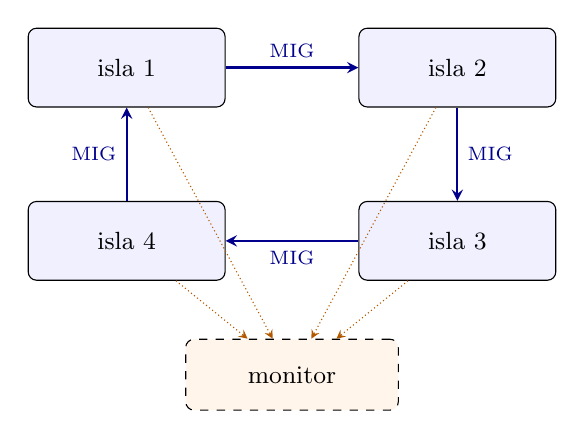
\begin{tikzpicture}[
  isl/.style={draw,rounded corners=3pt,minimum width=2.5cm,minimum height=1.0cm,
              fill=blue!6,font=\small},
  mon/.style={draw,dashed,rounded corners=3pt,minimum width=2.7cm,
              minimum height=0.9cm,fill=orange!8,font=\small},
  ar/.style={->,>=stealth,thick,blue!55!black},
  tel/.style={->,>=stealth,densely dotted,orange!70!black}]
  \node[isl] (a) at (0,0)      {isla 1};
  \node[isl] (b) at (4.2,0)    {isla 2};
  \node[isl] (c) at (4.2,-2.2) {isla 3};
  \node[isl] (d) at (0,-2.2)   {isla 4};
  \node[mon] (m) at (2.1,-3.9) {monitor};
  \draw[ar] (a) -- node[above,font=\scriptsize]{MIG} (b);
  \draw[ar] (b) -- node[right,font=\scriptsize]{MIG} (c);
  \draw[ar] (c) -- node[below,font=\scriptsize]{MIG} (d);
  \draw[ar] (d) -- node[left,font=\scriptsize]{MIG} (a);
  \foreach \i in {a,b,c,d} \draw[tel] (\i) -- (m);
\end{tikzpicture}
\caption{Arquitectura del cl\'uster.  Cuatro islas en anillo intercambian los
dos mejores genomas; cada isla env\'ia telemetr\'ia a un monitor independiente.
Las flechas continuas son migraci\'on; las punteadas, telemetr\'ia.}
\label{fig:arch}
\end{figure}

\subsection{Detalles de implementaci\'on}

Los n\'umeros aleatorios provienen de un generador xorshift \citep{marsaglia2003}
sembrado por isla.  El binario \texttt{langton-ga} tiene nueve subcomandos: \texttt{sim},
\texttt{analyze}, \texttt{evolve}, \texttt{island}, \texttt{monitor},
\texttt{demo}, \texttt{bench}, \texttt{render} y \texttt{help}.  Todo el c\'odigo
usa s\'olo \texttt{std}.  La evaluaci\'on paralela dentro de una isla emplea
\texttt{std::thread::scope} y divide la poblaci\'on en bloques contiguos, sin
canales ni \texttt{Arc} en el camino cr\'itico.  La comunicaci\'on usa sockets
TCP con timeouts de $500$\,ms y l\'ineas terminadas en salto de l\'inea, de modo
que el protocolo se puede inspeccionar con \texttt{nc}.  Las figuras se generan
sin bibliotecas gr\'aficas: un codificador PNG propio (bloques zlib
almacenados, CRC-32 y Adler-32) escribe las im\'agenes que aparecen en este
art\'iculo.

El Listado~\ref{lst:cli} muestra la invocaci\'on m\'inima de un cl\'uster de
cuatro islas y la reproducci\'on de un genoma concreto.

\begin{lstlisting}[language=bash,caption={Invocaci\'on del cl\'uster y
re-evaluaci\'on de un genoma.},label={lst:cli},numbers=none]
# cluster de 4 islas, 80 generaciones, migracion cada 5
./target/release/langton-ga demo --islands 4 --gens 80 --pop 64 \
    --steps 10000 --seed 1 --migration-interval 5 --migrants 2 \
    --states 2 --colors 3 --weights 0.20,0.20,0.50,0.10 \
    --base-port 8300 --out-dir results/distributed/m5_1

# re-evaluar el mejor genoma encontrado
./target/release/langton-ga analyze --states 2 --colors 3 --steps 60000 \
    --rule 020100000001020001020101020001010100
\end{lstlisting}

% ===========================================================================
\section{Metodolog\'ia experimental}\label{sec:method}
% ===========================================================================

\paragraph{Entorno.}
Todos los experimentos se ejecutaron en un Intel Core i5-8265U (4 n\'ucleos
f\'isicos, 8 hilos l\'ogicos) con 8\,GB de RAM, Linux 7.2 y Rust 1.99 en modo
\texttt{release}.  Cada isla usa un solo hilo; el modelo panm\'ictico usa cuatro.

\paragraph{Presupuesto.}
Todos los m\'etodos tienen el mismo presupuesto nominal: $4\times64\times80
=20\,480$ individuos-generaci\'on, cada uno simulado $T=10\,000$ pasos.  El
modelo secuencial y el panm\'ictico usan una poblaci\'on de $256$ y $80$
generaciones.  Las evaluaciones efectivas son algo menores porque los \'elites
se reutilizan sin re-simular: $\EvalsSeq$ en secuencial y panm\'ictico y
$\EvalsIsl$ en el cl\'uster (una diferencia del $2\%$).  La \'unica diferencia
real es c\'omo se reparte el trabajo.

\paragraph{Semillas y r\'eplicas.}
Cinco semillas por configuraci\'on ($1,\dots,5$).  En el cl\'uster, la semilla
$s$ genera las semillas de isla $100s+i$, de modo que cada r\'eplica arranca
poblaciones distintas y la ejecuci\'on es repetible salvo por el orden de
llegada de los mensajes.

\paragraph{M\'etricas.}
Se reportan: (i) la mejor aptitud final; (ii) el AUC de la curva de mejor
aptitud, $\frac{1}{G}\sum_g f_g$, que premia la rapidez de convergencia; (iii) el
tiempo hasta alcanzar $f=0{,}70$; (iv) la diversidad conductual final; (v) el
tiempo de pared; (vi) la aceleraci\'on $S_p=T_1/T_p$ y la eficiencia
$E_p=S_p/p$; y (vii) el tr\'afico de control.

\paragraph{Estad\'istica.}
Con cinco r\'eplicas usamos pruebas de permutaci\'on pareadas exactas
\citep{good2005}: se enumeran los $2^{5}=32$ cambios de signo de las diferencias
y se calcula la proporci\'on con media absoluta al menos la observada.  El
m\'inimo $p$ alcanzable es $2/32=0{,}0625$, por lo que el an\'alisis es
exploratorio; complementamos cada prueba con el tama\~no del efecto y con el
n\'umero de semillas en que un m\'etodo supera a otro.

\paragraph{Reproducibilidad.}
{\sloppy
El script \path{scripts/run_experiments.sh} ejecuta la suite completa y
\path{scripts/make_report.py} agrega los CSV y regenera tablas, figuras y
macros.  Los resultados crudos est\'an en \texttt{results/} y el PDF se compila
con \texttt{latexmk}.\par}

% ===========================================================================
\section{Resultados}\label{sec:results}
% ===========================================================================

\subsection{Validaci\'on con la regla cl\'asica}

La Tabla~\ref{tab:classic} confirma que el simulador y el detector reproducen el
comportamiento conocido.  La autopista aparece con per\'iodo $104$ y deriva
$(-2,2)$, una velocidad de $\ClassicSpeed$ celdas por paso y coincidencia
exacta del patr\'on trasladado ($\ClassicMatch$).  La Figura~\ref{fig:classic}
muestra el aspecto ca\'otico a los $12\,000$ pasos y la autopista ya formada a
los $120\,000$.  Obs\'ervese la densidad extremadamente baja
($\rho=\ClassicCompactness$): la autopista es una huella fina dentro de una caja
envolvente enorme, de $2163\times2135$ celdas.  Este es exactamente el tipo de
conducta que un objetivo de densidad puro penalizar\'ia, y justifica que la
aptitud combine varias se\~nales.

\begin{table}[t]
\centering
\caption{M\'etricas de la regla cl\'asica de Langton tras $120\,000$ pasos.}
\label{tab:classic}
\begin{tabular}{lr}
\toprule
M\'etrica & Valor \\
\midrule
Periodo de la autopista & 104 pasos \\
Deriva por periodo & (-2, 2) \\
Velocidad de traslaci\'on & 0.0272 celdas/paso \\
Coincidencia del patr\'on & 1.0000 \\
Celdas visitadas & 24652 \\
Revisitas & 95348 \\
Bounding box & 2163$\times$2135 \\
Movilidad & 0.0250 \\
Densidad & 0.0053 \\
Complejidad & 0.4824 \\
Vecindades 3$\times$3 & 247 \\
Aptitud (perfil balanced) & 0.186 \\
\bottomrule
\end{tabular}

\end{table}

\begin{figure}[t]
\centering
\begin{subfigure}[b]{0.44\linewidth}
  
\includegraphics[width=\linewidth]{classic_12k.png}
  \caption{$12\,000$ pasos: fase ca\'otica.}
\end{subfigure}\hfill
\begin{subfigure}[b]{0.54\linewidth}
  
\includegraphics[width=\linewidth]{classic_120k.png}
  \caption{$120\,000$ pasos: autopista.}
\end{subfigure}
\caption{Regla cl\'asica.  El color indica el n\'umero de visitas a cada celda.}
\label{fig:classic}
\end{figure}

\subsection{Convergencia en una sola isla}

Antes de distribuir la poblaci\'on conviene comprobar que el algoritmo
gen\'etico converge por s\'i solo.  La Figura~\ref{fig:single} muestra la
evoluci\'on con poblaci\'on $64$ y $80$ generaciones para dos perfiles.  El
perfil \emph{weaver} alcanza \SingleWeaverBest{} (cuatro semillas por encima de
$0{,}71$ y una en $0{,}625$), mientras que \emph{balanced} se estanca en
\SingleBalancedBest.  La diferencia no es de velocidad sino de \'optimo: el
perfil equilibrado converge r\'apidamente a una \'unica regla densa y estable
(desviaci\'on de $0{,}0004$), y el perfil de complejidad encuentra patrones
mejores pero con mucha m\'as varianza entre semillas.

\begin{figure}[t]
\centering
\begin{tikzpicture}
\begin{axis}[
  width=0.85\linewidth, height=5.8cm,
  xlabel={Generaci\'on}, ylabel={Mejor aptitud},
  xmin=0, xmax=79, ymin=0.35, ymax=0.78,
  grid=major, grid style={gray!18},
  legend pos=south east, legend cell align=left,
  legend style={font=\scriptsize,draw=gray!40},
  tick label style={font=\scriptsize}, label style={font=\small}]
  \addplot[blue!25,line width=0.4pt,forget plot] table[col sep=comma,x=gen,y=seed1]{data/single_weaver.csv};
  \addplot[blue!25,line width=0.4pt,forget plot] table[col sep=comma,x=gen,y=seed2]{data/single_weaver.csv};
  \addplot[blue!25,line width=0.4pt,forget plot] table[col sep=comma,x=gen,y=seed3]{data/single_weaver.csv};
  \addplot[blue!25,line width=0.4pt,forget plot] table[col sep=comma,x=gen,y=seed4]{data/single_weaver.csv};
  \addplot[blue!25,line width=0.4pt,forget plot] table[col sep=comma,x=gen,y=seed5]{data/single_weaver.csv};
  \addplot[blue!70!black,line width=1.1pt] table[col sep=comma,x=gen,y=mean]{data/single_weaver.csv};
  \addlegendentry{weaver}
  \addplot[orange!30,line width=0.4pt,forget plot] table[col sep=comma,x=gen,y=seed1]{data/single_balanced.csv};
  \addplot[orange!30,line width=0.4pt,forget plot] table[col sep=comma,x=gen,y=seed2]{data/single_balanced.csv};
  \addplot[orange!30,line width=0.4pt,forget plot] table[col sep=comma,x=gen,y=seed3]{data/single_balanced.csv};
  \addplot[orange!30,line width=0.4pt,forget plot] table[col sep=comma,x=gen,y=seed4]{data/single_balanced.csv};
  \addplot[orange!30,line width=0.4pt,forget plot] table[col sep=comma,x=gen,y=seed5]{data/single_balanced.csv};
  \addplot[orange!80!black,line width=1.1pt] table[col sep=comma,x=gen,y=mean]{data/single_balanced.csv};
  \addlegendentry{balanced}
\end{axis}
\end{tikzpicture}
\caption{Convergencia de una isla de $64$ individuos.  L\'ineas finas: semillas;
gruesas: media.  El perfil \emph{balanced} converge antes pero a una meseta
m\'as baja.}
\label{fig:single}
\end{figure}

\subsection{Comparaci\'on distribuida}

La Tabla~\ref{tab:distributed} compara los tres esquemas con el mismo
presupuesto nominal.  El cl\'uster de islas es $\SpeedupIsl\times$ m\'as r\'apido
que la versi\'on secuencial (eficiencia $\EfficiencyIsl\%$ sobre cuatro
procesos) y $\SpeedupPan\times$ m\'as r\'apido que el panm\'ictico con cuatro
hilos.  El tiempo hasta alcanzar $f=0{,}70$ resume la misma historia:
$\TSeventySeq$\,s en secuencial, $\TSeventyPan$\,s en panm\'ictico y $\TSeventyIsl$\,s en el
cl\'uster.

El secuencial y el panm\'ictico obtienen cifras \emph{id\'enticas}
(\FinalSeq{} y \FinalPan, AUC $\AucSeq$ y $\AucPan$, diversidad $\BdivSeq$ y
$\BdivPan$) porque ejecutan exactamente la misma b\'usqueda: la misma semilla
produce las mismas decisiones, y el paralelismo s\'olo cambia el tiempo.  Es una
comprobaci\'on \'util de que el planificador de hilos no altera la trayectoria
evolutiva.

El cl\'uster mejora ligeramente la calidad: \FinalIsl{} frente a \FinalSeq, un
$+0{,}023$ ($3{,}2\%$) que se observa en las cinco r\'eplicas.  Con cinco
semillas la prueba de permutaci\'on pareada no puede bajar de
$p=\PvalueIslPan$, de modo que el resultado debe leerse como una tendencia
consistente y no como una diferencia confirmada.  El AUC tambi\'en es superior
($\AucIsl$ frente a $\AucSeq$): el cl\'uster no s\'olo llega un poco m\'as lejos,
sino que progresa antes.  La diversidad conductual tard\'ia es claramente mayor
($\BdivIsl$ frente a $\BdivSeq$), en l\'inea con la idea de que varias
subpoblaciones independientes exploran cuencas distintas; en una de las
r\'eplicas secuenciales la poblaci\'on colapsa a una diversidad de $0{,}16$,
mientras que ninguna isla baja de $0{,}79$.  La
Figura~\ref{fig:convergence} muestra las curvas completas: las l\'ineas finas
son las cinco semillas y la gruesa su media.

\begin{table}[t]
\centering
\caption{Comparaci\'on de los tres esquemas de ejecuci\'on con el mismo
presupuesto nominal ($T=10\,000$).  Media $\pm$ desviaci\'on sobre cinco
semillas.  La diversidad conductual es la media de las \'ultimas $16$
generaciones.}
\label{tab:distributed}
\resizebox{\linewidth}{!}{\begin{tabular}{lrrrrrr}
\toprule
Modo & Tiempo (s) & Acel. & Evaluaciones & Mejor final & AUC & Div. conductual \\
\midrule
Secuencial & 18.98 & 1.00 & 20322 & $0.714 \pm 0.014$ & 0.683 & 0.697 \\
Panm\'ictico & 7.88 & 2.41 & 20322 & $0.714 \pm 0.014$ & 0.683 & 0.697 \\
Islas (m=5) & 6.05 & 3.14 & 19919 & $0.737 \pm 0.012$ & 0.711 & 0.899 \\
\bottomrule
\end{tabular}
}
\end{table}

\begin{figure}[t]
\centering
\begin{tikzpicture}
\begin{axis}[
  width=0.92\linewidth, height=6.6cm,
  xlabel={Generaci\'on}, ylabel={Mejor aptitud},
  xmin=0, xmax=79, ymin=0.40, ymax=0.78,
  grid=major, grid style={gray!18},
  legend pos=south east, legend cell align=left,
  legend style={font=\scriptsize,draw=gray!40},
  tick label style={font=\scriptsize}, label style={font=\small}]
  % --- sequential: five faint seeds
  \addplot[gray!30,line width=0.4pt,forget plot] table[col sep=comma,x=gen,y=seed1]{data/dist_seq.csv};
  \addplot[gray!30,line width=0.4pt,forget plot] table[col sep=comma,x=gen,y=seed2]{data/dist_seq.csv};
  \addplot[gray!30,line width=0.4pt,forget plot] table[col sep=comma,x=gen,y=seed3]{data/dist_seq.csv};
  \addplot[gray!30,line width=0.4pt,forget plot] table[col sep=comma,x=gen,y=seed4]{data/dist_seq.csv};
  \addplot[gray!30,line width=0.4pt,forget plot] table[col sep=comma,x=gen,y=seed5]{data/dist_seq.csv};
  \addplot[black,line width=1.1pt] table[col sep=comma,x=gen,y=mean]{data/dist_seq.csv};
  \addlegendentry{Secuencial}
  % --- panmictic
  \addplot[blue!35,line width=0.4pt,forget plot] table[col sep=comma,x=gen,y=seed1]{data/dist_pan.csv};
  \addplot[blue!35,line width=0.4pt,forget plot] table[col sep=comma,x=gen,y=seed2]{data/dist_pan.csv};
  \addplot[blue!35,line width=0.4pt,forget plot] table[col sep=comma,x=gen,y=seed3]{data/dist_pan.csv};
  \addplot[blue!35,line width=0.4pt,forget plot] table[col sep=comma,x=gen,y=seed4]{data/dist_pan.csv};
  \addplot[blue!35,line width=0.4pt,forget plot] table[col sep=comma,x=gen,y=seed5]{data/dist_pan.csv};
  \addplot[blue!70!black,line width=1.1pt] table[col sep=comma,x=gen,y=mean]{data/dist_pan.csv};
  \addlegendentry{Panm\'ictico (4 hilos)}
  % --- islands m5
  \addplot[red!35,line width=0.4pt,forget plot] table[col sep=comma,x=gen,y=seed1]{data/dist_m5.csv};
  \addplot[red!35,line width=0.4pt,forget plot] table[col sep=comma,x=gen,y=seed2]{data/dist_m5.csv};
  \addplot[red!35,line width=0.4pt,forget plot] table[col sep=comma,x=gen,y=seed3]{data/dist_m5.csv};
  \addplot[red!35,line width=0.4pt,forget plot] table[col sep=comma,x=gen,y=seed4]{data/dist_m5.csv};
  \addplot[red!35,line width=0.4pt,forget plot] table[col sep=comma,x=gen,y=seed5]{data/dist_m5.csv};
  \addplot[red!75!black,line width=1.1pt] table[col sep=comma,x=gen,y=mean]{data/dist_m5.csv};
  \addlegendentry{Islas ($g=5$)}
\end{axis}
\end{tikzpicture}
\caption{Convergencia de la mejor aptitud.  L\'ineas finas: semillas
individuales; l\'ineas gruesas: media de cinco semillas.}
\label{fig:convergence}
\end{figure}

\begin{table}[t]
\centering
\caption{Efecto del intervalo de migraci\'on $g$ en el cl\'uster de cuatro
islas ($0$ = sin migraci\'on).  Media $\pm$ desviaci\'on sobre cinco semillas;
la diversidad es la media de las \'ultimas $16$ generaciones.}
\label{tab:migration}
\begin{tabular}{rrrrrr}
\toprule
Intervalo & Mejor final & AUC & Div. conductual & Tiempo (s) & Control (KB) \\
\midrule
0 & $0.736 \pm 0.008$ & 0.703 & 0.869 & 5.51 & 14.2 \\
5 & $0.737 \pm 0.012$ & 0.711 & 0.899 & 6.05 & 19.0 \\
20 & $0.737 \pm 0.012$ & 0.702 & 0.877 & 5.95 & 15.2 \\
\bottomrule
\end{tabular}

\end{table}

\subsection{Ablaci\'on del intervalo de migraci\'on}

La Tabla~\ref{tab:migration} y la Figura~\ref{fig:migration} estudian el efecto
del intervalo de migraci\'on.  Sin migraci\'on ($g=0$) las cuatro islas
evolucionan de forma independiente; la diversidad conductual tard\'ia es
$\MigNoneBdiv$ y pasa a $\MigFiveBdiv$ con $g=5$ y a $\MigTwentyBdiv$ con $g=20$.  La
mejor aptitud final es pr\'acticamente la misma en los tres reg\'imenes:
\MigNoneBest{} sin migraci\'on, \MigFiveBest{} con $g=5$ y \MigTwentyBest{} con $g=20$.
Las diferencias no son significativas ($p=\PvalueMigNoneFive$ entre $g=0$ y $g=5$;
$p=\PvalueMigFiveTwenty$ entre $g=5$ y $g=20$) y el tama\~no del efecto es
despreciable.

La explicaci\'on es estructural: el m\'aximo del cl\'uster es el m\'aximo sobre
cuatro islas, y el paisaje de aptitud tiene unos pocos atractores fuertes.  Un
pu\~nado de reglas ($0{,}7445$, $0{,}7291$, $0{,}7258$) explica la mayor\'ia de
los finales de las quince ejecuciones, de modo que basta con que \emph{una} isla
encuentre el atractor para fijar el m\'aximo; la migraci\'on no puede mejorarlo.
Su efecto se observa, si acaso, en la diversidad ($p=\PvalueDivMigNoneFive$, no
significativo) y en el tr\'afico de control, que pasa de $\MigNoneKb$\,KB sin
migraci\'on a $\MigFiveKb$\,KB con $g=5$ (el resto es telemetr\'ia: un mensaje por
isla y generaci\'on).

\begin{figure}[t]
\centering
\begin{tikzpicture}
\begin{axis}[
  width=0.62\linewidth, height=5.4cm,
  ybar, bar width=16pt,
  xlabel={Intervalo de migraci\'on $g$ (generaciones)},
  ylabel={Mejor aptitud final},
  xmin=-2, xmax=22, ymin=0.68, ymax=0.77,
  xtick={0,5,20}, xticklabels={sin migraci\'on,5,20},
  grid=major, grid style={gray!18},
  tick label style={font=\scriptsize}, label style={font=\small}]
  \addplot[fill=blue!35,draw=blue!60!black,
           error bars/.cd,y dir=both,y explicit]
    table[col sep=comma,x=interval,y=best_mean,y error=best_sd]{data/migration.csv};
\end{axis}
\end{tikzpicture}
\caption{Aptitud final media ($\pm$ desviaci\'on) seg\'un el intervalo de
migraci\'on.}
\label{fig:migration}
\end{figure}

\subsection{Portafolio heterog\'eneo}

El experimento m\'as ilustrativo cualitativamente es el portafolio: cuatro islas
con perfiles de pesos distintos y sin migraci\'on, $60$ generaciones.  La
Tabla~\ref{tab:portfolio} resume los mejores genomas y la
Figura~\ref{fig:gallery} muestra los patrones.  Cada perfil encuentra una
conducta diferente:
\begin{itemize}
  \item \textbf{Mover} ($w_m=0{,}80$) produce un deslizador diagonal: una
        autopista de per\'iodo $8$ con deriva $(4,-4)$, es decir
        $\PortfolioMoverSpeed$ celdas por paso, y s\'olo tres vecindades
        $3\times3$ distintas.  Es movilidad pura.
  \item \textbf{Builder} ($w_\rho=0{,}75$) construye una banda densa de dos
        filas que llena el $99{,}9\%$ de su caja envolvente y se desplaza
        lentamente (per\'iodo $10$, deriva $(0,2)$).  Al igual que la cinta, es
        una estructura cuasi unidimensional: la densidad se maximiza
        ``adelgazando'' el patr\'on hasta una franja.
  \item \textbf{Weaver} ($w_\kappa=0{,}50$) genera un patr\'on ramificado y
        est\'atico con $1548$ vecindades $3\times3$ distintas y movilidad
        pr\'acticamente nula.
  \item \textbf{Balanced} descubre una cinta transportadora de per\'iodo $9$ y
        deriva $(0,3)$: un caso intermedio entre transporte y estructura, con
        movilidad $0{,}333$ y densidad alta.
\end{itemize}

Los cuatro genomas tienen aptitud alta \emph{bajo su propio perfil} (entre
$\PortfolioBalancedFit$ y $\PortfolioBuilderFit$), pero al re-evaluarlos con el
perfil \emph{weaver} solo el tejedor conserva un valor alto ($0{,}689$): el
constructor cae a $0{,}345$, el equilibrado a $0{,}336$ y el deslizador a
$0{,}211$.  Los perfiles no son variaciones cosm\'eticas del mismo objetivo:
inducen regiones diferentes del espacio de reglas.

\begin{table}[t]
\centering
\caption{Portafolio heterog\'eneo: mejor genoma por perfil tras $60$
generaciones.  La \'ultima columna indica per\'iodo y deriva cuando el
an\'alisis detecta una autopista.}
\label{tab:portfolio}
\resizebox{\linewidth}{!}{\begin{tabular}{lrrrrrrr}
\toprule
Perfil & Aptitud & Apt.\ weaver & Movilidad & Densidad & Compl. & Vec. & Per.\ / deriva \\
\midrule
mover & 0.633 & 0.211 & 0.7071 & 0.000 & 0.006 & 3 & 8 / (4,-4) \\
builder & 0.861 & 0.345 & 0.2000 & 1.000 & 0.010 & 5 & 10 / (0,2) \\
weaver & 0.707 & 0.689 & 0.0014 & 0.445 & 1.000 & 1548 & --- \\
balanced & 0.484 & 0.336 & 0.3333 & 1.000 & 0.006 & 3 & 9 / (0,3) \\
\bottomrule
\end{tabular}
}
\end{table}

\begin{figure}[t]
\centering
\begin{subfigure}[b]{0.36\linewidth}
  \centering
  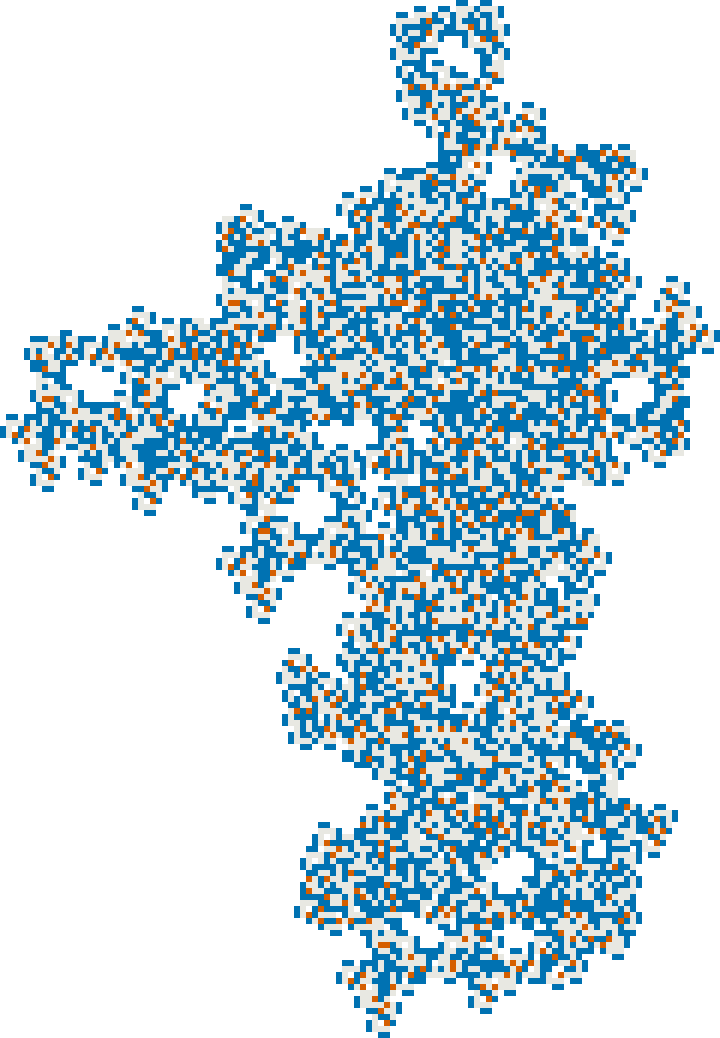
\includegraphics[height=5.2cm]{weaver.png}
  \caption{Tejedor ($w_\kappa=0{,}50$)}
\end{subfigure}\hfill
\begin{subfigure}[b]{0.58\linewidth}
  \centering
  
\includegraphics[height=5.2cm]{mover.png}
  \caption{Deslizador diagonal ($w_m=0{,}80$)}
\end{subfigure}

\vspace{0.6em}
\begin{subfigure}[b]{0.98\linewidth}
  \centering
  \begin{tikzpicture}
  \begin{axis}[
    width=0.94\linewidth, height=4.3cm,
    xlabel={Paso}, ylabel={Desplazamiento},
    xmin=0, xmax=2000, ymin=0, ymax=3000,
    grid=major, grid style={gray!18},
    legend pos=north west, legend cell align=left,
    legend style={font=\scriptsize,draw=gray!40},
    tick label style={font=\scriptsize}, label style={font=\small}]
    \addplot[blue!70!black,line width=0.9pt] table[col sep=comma,x=step,y=displacement]{data/traj_mover.csv};
    \addlegendentry{mover}
    \addplot[orange!85!black,line width=0.9pt] table[col sep=comma,x=step,y=displacement]{data/traj_builder.csv};
    \addlegendentry{builder}
    \addplot[green!45!black,line width=0.9pt] table[col sep=comma,x=step,y=displacement]{data/traj_balanced.csv};
    \addlegendentry{balanced}
    \addplot[purple,line width=0.9pt] table[col sep=comma,x=step,y=displacement]{data/traj_weaver.csv};
    \addlegendentry{weaver}
  \end{axis}
  \end{tikzpicture}
  \caption{Desplazamiento acumulado: transporte lineal frente a patr\'on localizado}
\end{subfigure}
\caption{Conductas descubiertas por el portafolio heterog\'eneo.  (a,b)~Patrones
finales; el color codifica el n\'umero de visitas.  (c)~Distancia al origen en
funci\'on del tiempo para las cuatro reglas.}
\label{fig:gallery}
\end{figure}

\subsection{Rendimiento del simulador}

La Tabla~\ref{tab:bench} resume el costo de una evaluaci\'on aislada
($T=20\,000$, 100 iteraciones).  El simulador procesa
$\BenchMillionsSteps$ millones de pasos por segundo en un n\'ucleo, lo que
explica que una generaci\'on de $64$ individuos con $T=10^{4}$ tarde del orden de
$0{,}05$\,s en un n\'ucleo.  La rejilla dispersa y la ausencia de asignaciones en el camino
caliente son responsables de esta cifra.

\begin{table}[t]
\centering
\caption{Rendimiento de la evaluaci\'on (un n\'ucleo, $T=20\,000$,
100 repeticiones).}
\label{tab:bench}
\begin{tabular}{lr}
\toprule
M\'etrica & Valor \\
\midrule
Evaluaciones por segundo & 606.6 \\
Pasos de simulaci\'on por segundo & 12\,131\,175 \\
Millones de pasos por segundo & 12.13 \\
Celdas visitadas por segundo & 2\,120\,529 \\
\bottomrule
\end{tabular}

\end{table}

% ===========================================================================
\section{Discusi\'on}\label{sec:discussion}
% ===========================================================================

\paragraph{\texorpdfstring{¿Por qu\'e el cl\'uster solo mejora ligeramente?}{Por que el cluster solo mejora ligeramente?}}
El cl\'uster reparte el presupuesto en cuatro subpoblaciones de $64$ durante
$80$ generaciones, mientras que el panm\'ictico concentra $256$ individuos en
una sola bolsa gen\'etica.  La migraci\'on ocurre solo $16$ veces ($g=5$), de
modo que cada isla explora la mayor parte del tiempo por su cuenta; el efecto
observado es una mejora peque\~na pero consistente ($+3{,}2\%$, cinco de cinco
r\'eplicas) y una diversidad tard\'ia mucho mayor.  La interpretaci\'on
razonable es que las islas conservan varias cuencas de atracci\'on y que el
m\'aximo sobre cuatro poblaciones aprovecha esa exploraci\'on, mientras que la
poblaci\'on panm\'ictica converge m\'as r\'apido a un \'unico atractor.  Con un
paisaje tan peque\~no y solo cinco semillas no es posible separar este efecto
del azar; para ello har\'ian falta m\'as r\'eplicas o un espacio de b\'usqueda
mayor.  La ventaja m\'as s\'olida del cl\'uster es de \emph{ingenier\'ia}: el
mismo resultado en un tercio del tiempo y la posibilidad de crecer a varias
m\'aquinas.

\paragraph{Diversidad y especializaci\'on.}
El portafolio muestra que la diversidad no es un adorno: con cuatro perfiles se
obtienen cuatro morfolog\'ias que un \'unico objetivo escalar no visitar\'ia.
Esto conecta con la literatura de novedad y calidad-diversidad
\citep{lehman2011} y sugiere una extensi\'on natural: usar la diversidad
conductual como criterio de selecci\'on o de archivo, en lugar de s\'olo como
m\'etrica.

\paragraph{La aptitud como hip\'otesis.}
Los resultados dependen fuertemente de los pesos.  El perfil \emph{balanced}
aumenta la movilidad y la complejidad a costa de la densidad, y por eso
redescubre una cinta; el perfil \emph{weaver} prioriza complejidad y produce
patrones est\'aticos.  No hay una aptitud ``correcta'': hay una familia de
hip\'otesis sobre qu\'e hace interesante a una regla, y el marco permite
contrastarlas con el mismo presupuesto.

\paragraph{Amenazas a la validez.}
(i)~Cinco semillas dan una potencia estad\'istica baja: el $p$ m\'inimo de una
prueba de permutaci\'on pareada es $0{,}0625$, insuficiente para el umbral
convencional de $0{,}05$.  Reportamos tama\~nos de efecto y direcciones, no
s\'olo valores $p$.  (ii)~Los experimentos se hicieron en una sola m\'aquina con
cuatro n\'ucleos f\'isicos; la aceleraci\'on no refleja latencias de red reales.
(iii)~El tr\'afico de control reportado incluye la telemetr\'ia (un mensaje por
generaci\'on), que domina el total; el payload de migraci\'on es de $\sim\!72$
bytes por evento.  (iv)~La complejidad es una estimaci\'on por filtro de Bloom.
(v)~Las ejecuciones del cl\'uster no son reproducibles bit a bit por la
naturaleza as\'incrona de la red; s\'i lo son las locales.  (vi)~El detector de
autopistas exige coincidencia exacta en una ventana de radio $128$; patrones
m\'as grandes podr\'ian escaparse.  (vii)~Las islas arrancan con semillas
derivadas ($100s+i$) distintas de las del secuencial y el panm\'ictico, de modo
que la comparaci\'on emparejada por \'indice de r\'eplica no usa n\'umeros
aleatorios comunes; los tama\~nos de efecto deben interpretarse con cautela.

% ===========================================================================
\section{Conclusiones y trabajo futuro}\label{sec:conclusions}
% ===========================================================================

Construimos un sistema completo ---modelo, simulador, aptitud, algoritmo
gen\'etico, cl\'uster TCP, monitor, figuras y suite experimental--- para evolucionar
turmites de Langton y lo evaluamos con un protocolo reproducible.  El cl\'uster
de islas iguala o mejora ligeramente la calidad del panm\'ictico con una
aceleraci\'on de $\SpeedupIsl\times$ sobre la versi\'on secuencial y una
eficiencia del $\EfficiencyIsl\%$, y el portafolio heterog\'eneo redescubre
cuatro familias de conducta, incluida una cinta transportadora de per\'iodo $9$;
la autopista cl\'asica de per\'iodo $104$ se usa como validaci\'on del detector.  El c\'odigo, los
datos crudos y los scripts permiten regenerar cada tabla y figura.

El trabajo futuro se orienta en cuatro direcciones: (i)~selecci\'on por
diversidad conductual o archivo de novedad, para evitar la convergencia de las
islas; (ii)~migraci\'on adaptativa, con intervalo y n\'umero de migrantes
dependientes de la heterogeneidad medida; (iii)~topolog\'ias distintas del anillo
(grafo completo, malla, \emph{gossip}) y comparaci\'on sistem\'atica; y
(iv)~ejecuci\'on en varias m\'aquinas con fallos y latencias reales, que es donde
el modelo distribuido deber\'ia mostrar su ventaja.

\appendix
\section{Reproducci\'on}

\begin{lstlisting}[language=bash,caption={Secuencia completa de
reproducci\'on.},label={lst:repro},numbers=none]
cargo build --release
cargo test --release                     # 22 pruebas
./scripts/run_experiments.sh             # resultados crudos
python3 scripts/make_report.py           # tablas, macros y figuras
cd paper && latexmk -pdf main.tex        # este documento
\end{lstlisting}

La correspondencia entre artefactos y secciones es la siguiente:
\texttt{results/baseline/} alimenta la Tabla~\ref{tab:classic} y la
Figura~\ref{fig:classic}; \texttt{results/distributed/} alimenta las
Tablas~\ref{tab:distributed}--\ref{tab:migration} y las
Figuras~\ref{fig:convergence}--\ref{fig:migration};
\texttt{results/portfolio/} y \texttt{results/gallery/} alimentan la
Tabla~\ref{tab:portfolio} y la Figura~\ref{fig:gallery}.  Los CSV agregados
est\'an en \texttt{paper/data/}, las tablas en \texttt{paper/tables/} y las
figuras en \texttt{paper/figs/}.

{\small
\bibliographystyle{plainnat}
\bibliography{refs}
}

\end{document}
